\documentclass[11pt,border=5pt]{standalone}
\usepackage{fontspec}
\setmainfont{cmunrm.otf}[BoldFont=cmunbx.otf,ItalicFont=cmunti.otf,BoldItalicFont=cmunbi.otf]
\usepackage{amsmath}
\usepackage{unicode-math}
\setmathfont{NewCMMath-Regular.otf}
\usepackage{tikz}
\usetikzlibrary{arrows.meta,patterns,angles,quotes}
\begin{document}
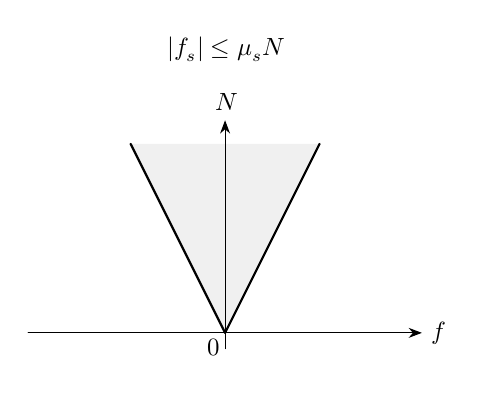
\begin{tikzpicture}[>=Stealth,font=\small,line cap=round,line join=round]
\draw[->,thin] (-2.5,0) -- (2.5,0) node[right] {$f$};
\draw[->,thin] (0,-0.2) -- (0,2.7) node[above] {$N$};
\node at (-0.14,-0.18) {$0$};
\draw[thick] (0,0) -- (1.2,2.4);
\draw[thick] (0,0) -- (-1.2,2.4);
\fill[black,opacity=.06] (0,0)--(1.2,2.4)--(-1.2,2.4)--cycle;\node at (0,3.6) {$|f_s|\le\mu_s N$};

\end{tikzpicture}
\end{document}
